%!TEX root = ../template.tex
%%%%%%%%%%%%%%%%%%%%%%%%%%%%%%%%%%%%%%%%%%%%%%%%%%%%%%%%%%%%%%%%%%%%
%% chapter2.tex
%% NOVA thesis document file
%%
%% Chapter with the template manual
%%%%%%%%%%%%%%%%%%%%%%%%%%%%%%%%%%%%%%%%%%%%%%%%%%%%%%%%%%%%%%%%%%%%

\typeout{NT FILE chapter2.tex}%

\newcommand{\cmark}{\ding{51}}%
\newcommand{\xmark}{\ding{55}}%

\chapter{Background}
\label{cha:background}

In this chapter we address some relevant issues for the background of this dissertation. We begin with an overview of a \gls{DL} (section \ref{sec:background:decentralized_ledgers}) and discussing the different models of a blockchain (section \ref{sec:background:blockchain_models}). Next, we present smart contracts (section \ref{sec:background:smart_contracts}) with a comparative analysis of their implementation by various blockchain platforms. Additionally, we present the architecture of a blockchain and the different planes that compose it, with focus on the used consensus mechanisms and their limitations/tradeoffs (section \ref{sec:background:arch_service_planes}). % Then, in section \ref{sec:background:comparison-blockchain} we compare different blockchain systems focused on the consensus plane.
Finally, in section \ref{sec:background:summary} we present a summary of this chapter.



\section{Decentralized Ledgers}
\label{sec:background:decentralized_ledgers}

A Decentralized Ledger (\gls{DL}) is a Data Storage Technology in which the data is replicated and accessible across many nodes. In contrast to a centralized database, a \gls{DL} fits in an architecture that does not require a central administrator to process, validate or authenticate transactions, and consequently does not have a single point of failure. By their nature, these types of systems provide high availability with the possibility to combine the resources from multiple nodes for greater storage capacity and higher concurrent access. However, due to the fact that this type of system operates on a distributed setting, it is required to solve the consensus problem so that the ledger is correctly replicated through all of the participating nodes. Moreover, all the records in the ledger are timestamped and signed with a cryptographic algorithm, providing a way to verify and audit the history of the stored data.

A blockchain is essentially a specific type of \gls{DL} that implements a secure, unmodifiable and append-only log of transactions. In this initial definition the word “transaction” is used in a broad sense. For example, in Bitcoin \cite{bitcoin}, a transaction is just a transfer of cryptocurrency value between two accounts with anonymous identifiers, where any node can join the system. In other blockchains, transactions do not necessarily involve money transfers and can be used to support trades of digital assets by using smart contracts. Additionally, a blockchain can be seen as a possible organization of a distributed database, in which different nodes manage locally replicated logs of transactions and related shared state, with given guarantees of consistency, availability, and network partition tolerance. Next, we present the main characteristics of a blockchain system \cite{the_blockchain_state_of_the_art}:

% There are many types of \gls{DL} and a Blockchain is one of them in the sense that it represents a Data Structure comprised of blocks in which a block contains a set of transactions (in section \ref{sec:rel_work:dl_ds} is performed a more focused and deeper understanding of different \gls{DL}'s structures). In this particular implementation, the allowed data operations are: 1) get any block in the chain given its identifier (a hash of the block) and 2) insert a new validated block. Due to this approach of not having a remove block operation, a blockchain consists of an immutable data structure in which blocks can only be appended to it. Thus, the main characteristics of a blockchain system are \cite{the_blockchain_state_of_the_art}:

\begin{itemize}
    \item Decentralization: Every node has the ability to get any block or to append one to the chain, unlike centralized systems that are controlled by a centralized authority;
    \item Detrusting: Data transfer between two nodes in the network does not require mutual trust, based on the fact that all transactions are stored in blocks and the blockchain uses a hash function with a consensus mechanism to add new blocks to the chain;
    \item Transparency: Every node has the ability to query blocks and transactions in the system, thus the information is transparent and consistent;
    \item Traceable and unforgeable: The use of timestamps in each transaction allows to keep an order of transactions (traceable) and once added to the chain it cannot be tampered with, thus making it unforgeable.
    \item Anonymity: It is not necessary to disclose the true identity of the participant, instead public keys based on asymmetric encryption are used for anonymous identification;
    \item Credibility: Each node stores the complete data and the operation of adding a block is done under conditions of anonymity, thus protecting privacy of all participants and credibility of transactions.
\end{itemize}

% \begin{itemize}
%     \item Decentralization: Since a blockchain is based on a Decentralized System, decentralization is guaranteed in the sense that every node has the ability to get any block or to append one to the chain, unlike centralized systems that are controlled by a centralized authority.
%     \item Detrusting: Data transfer between two nodes in the network does not require mutual trust, based on the fact that decentralization is a feature of this system and the use of decentralized structures form a trust relationship between the participating nodes and the system. Since all transactions are stored in blocks and the blockchain uses a hash function with a consensus mechanism to add new blocks to the chain we can consider a transaction to be detrusting.
%     \item Transparency: Every node has the ability to query blocks and transactions in the system, thus the information is transparent and consistent. This ensures that a transaction data is open and reliable.
%     \item Traceable and unforgeable: The use of timestamps in each transaction allows to keep an order of transactions and to make them traceable. Also, when a transaction is validated and added to a block of the chain it cannot be tampered with, thus making it unforgeable.
%     \item Anonymity: A Blockchain uses asymmetric encryption for two cases: data encryption to ensure the security of the transaction data and digital signatures to be able to identify the signatory and validate the transaction. In this system, it is not necessary to disclose the true identity of the participant and so, it respects anonymity.
%     \item Credibility: Each node stores the complete data and the operation of adding a block is done under conditions of anonymity, thus protecting privacy of all participants and credibility of transactions.
% \end{itemize}

% In relation to a block, along with the transactions (data) there is a $previous$ field that indicates the previous block in the chain and so, the blockchain can be seen as a tree of blocks. The first block of a blockchain (the root of the tree) is a special block without any transactions which is called the genesis block and consequently, does not have a previous block. In section \ref{sec:rel_work:dl_ds} is performed a more focused and deeper understanding of \gls{DL}'s structures, such as: finalization of blocks and weight use, the DAG block models and the concept of decoupling consensus from the dissemination of blocks in the network.


\section{Blockchain Models as Decentralized Ledgers}
\label{sec:background:blockchain_models}

There are many types or models for blockchains that are related to the nature, characteristics, and targeted applications. A model indicates how data is accessed (access-control) and the permissions for each participant. Blockchains are in general typified in the literature in different categories and terminology, corresponding to the following models: permissioned blockchains, permissionless blockchains, consortium blockchains, private blockchains, public blockchains or hybrid blockchains. % When building or using an existing Blockchain, the choice of a specific model is necessary and is dependent on the application domains, characteristics and strategies.

% Depending on the nature, characteristics, and targeted applications, blockchains are in general typified in the literature in different categories and terminology: permissioned blockchains, permissionless blockchains, consortium-blockchains, private blockchains, public blockchains or hybrid blockchains. Characterizations of such types are presented as follow:

\begin{figure}[h]
    \centering
    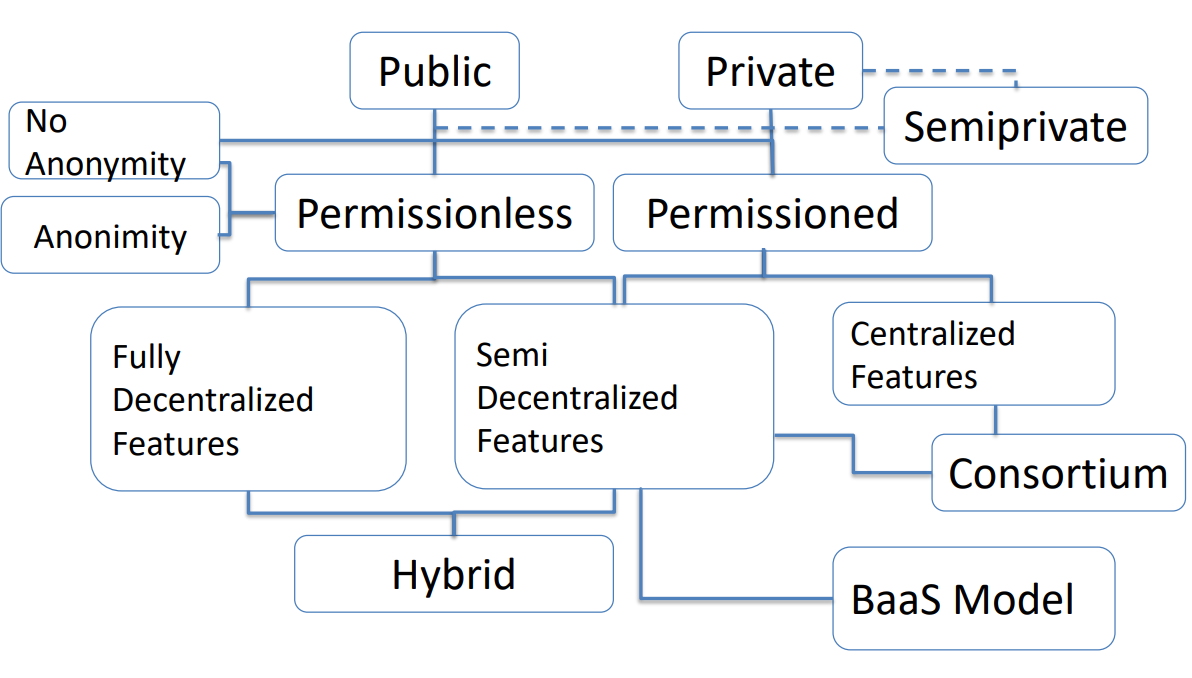
\includegraphics[scale=0.3]{Chapters/Figures/blockchain_models_framework.png}
    \caption{Blockchain Models Framework}
    \label{fig:blockchain_models_framework}
\end{figure}

In figure \ref{fig:blockchain_models_framework} is represented a framework to classify different blockchains according to the different models \cite{systematic_survey_blockchain_systems} which are presented as follows. % Blockchains can be divided in three main models: public, private and hybrid.  % Firstly, blockchains can be divided into two models: public and private. Secondly, in each of these models, they fit in a permissionless or permissioned settings. Lastly there are two other models that solve the drawbacks of the other models, such as: Hybrid and Consortium or Federated models.



\paragraph{Public Model}

In the public model there is no central authority in the system, in the sense that every participant is able to read, write, verify and enter in the consensus protocol of the data on the chain. In this model, anyone can join as a node in the system without the need for being approved, which helps to achieve a self-governed and decentralized nature as permissionless ledgers or permissionless blockchains, with the facets introduced below. % According to figure \ref{fig:blockchain_models_framework}, the \textbf{Permissionless} category can be applied to both public and private models. However, the main use of this model is in the context of the public one.

\paragraph{Permissionless Model}

The permissionless category represents a fully decentralized blockchain where anyone can read the data and host a node anonymously without the need to be approved. For this purpose, these blockchains are based on open-source and transaparent code, allowing any participant to install and deploy its own network node. In this way, any user can validate transactions and decide the state of the \gls{DL} that follows consistency rules based on consensus mechanisms defined by the code and runtime execution. In the context of this dissertation, we are particularly interested on permissionless blockchains, in which we emphasize the following aspects from our related work study:  % The first blockchains are based on this model and Bitcoin is an example of such system where each node receive an incentive (currently 6,25 BTC) each time a block is added to the chain through mining. An important note on this type of systems is that the transaction approval is in order of minutes. The main characteristics of this model are:

\begin{itemize}
    \item Permissionless operation: All participants are able to create and disseminate transactions where any one has equal access to validate transactions and to create, propose and validate blocks, following the same rules. For this purpose, it is required a consistent model for the verification of blocks that is related to the block finalization concept in such blockchains. Additionally, these blockchains have been the field for the support of many cryptocurrencies where block finalization requires consensus mechanisms that are related to the notion of "mining"~for successful proposers;
    \item Block mining, finalization and incentivation: Any participant can create and propose blocks that must be verifiable by a certain number or majority of other participants, for security guarantees. In this case, blocks (and consequently their transactions) are finalized with a certain amount of cryptocurrency value being assigned to the miner as the incentive. This incentive is the way to create cryptocurrency value;
    \item Finalization with unknown participants: In permissionless blockchains, it is interesting to relate the block finalization with solving the consensus problem in a large-scale settings and in a network of unknown participants. In fact, these systems employ a dynamic membership approach in which participants can enter or exit the system at any time. Therefore, consensus solutions must address the required guarantees for safety and liveness conditions under the \gls{CUP} model with an impact on tradeoffs between consistency, security and performance, including throughput and latency metrics for finality guarantees. Not surprisingly, different mechanisms used to solve consensus in a \gls{CUP} model under scalable conditions and performance requirements can strongly influence the operation of the consensus plane of different blockchains and permissionless ledger models.
    % \item Anonymity: All participants are possible anonymous with unauthenticated communication;
    % \item High scalability: The number of participants in these systems may be uncertain due to the fact that the system is open and any user can enter in the protocol, thus being able to achieve millions of participants;
    % \item Byzantine behaviour: Since the system is permissionless anyone can access it anonymously, thus there is the possibility of some nodes to have a byzantine behaviour, i.e. nodes that do not follow the protocol. As such, blockchains must be able to detect and mitigate the actions (attacks) of these incorrect participants, such as: having consensus mechanisms that are \gls{BFT}, like \gls{PoW} and possibly some kind of penalization system to reduce the probability of attack like in Ethereum where the staked capital of the attacker is revoked \cite{ethereum_penalties};
    % \item Dynamic membership: Nodes can enter or exit the system at any time.
\end{itemize}

% By contrast, the \textbf{private permissionless model} only allows pre-approved nodes to participate and validate transactions. Additionally, all nodes continue to be anonymous. 

\paragraph{Permissioned Model}

In the permissioned model, only approved participants can join the system. The membership is typically established and defined by deployment and configurations as a management process, allowing for refined control over the blockchain. In general, there is also an access control of who has the write to finalize blocks and obtain the reward. In contrast to permissionless blockchains, the number of nodes is much more reduced and the risk of byzantine behaviour is almost negligible. This allows for choosing a more efficient and traditional consensus mechanism where there is no need for costly mining, like \gls{PoW}. Consequently, the efficiency of this type of blockchain is much higher than the permissionless one, where the transaction approval can be reduced to an order of milliseconds. In fact, there are two categories that are inserted in this model, such as: \textbf{Private} and \textbf{Consortium or Federated}.

% A permissioned system is controlled by one authority which ensures a certain degree of trust (HyperLedger, Tendermint, Chain and Quorum \cite{hyperleder_fabric, tendermint, chain, quorum} are examples of such systems). In fact, this model describes a centralized chain where there is a whitelist of allowed users (known identities) with particular characteristics and permissions over the operations on the network.

In \textbf{Private blockchains}, the access is restricted to authorized participants with the government and operation usually associated to a single entity which ensures a certain degree of trust. This type of blockchains are designed to target specific business requirements with high level of security guarantees and management control. A typical scenario for private blockchains is the support of internal processes for an organization or company, where a decentralized, trustable, and secure ledger is needed for tracking and recording data.

In addition to private systems, there are other solutions that try to extend that category to be able to integrate multiple organizations known as \textbf{Consortium or Federated systems}. In this type of systems, the operation to add a new block to the chain is determined by a set of pre-selected or leader nodes and it shares a similar scalability and privacy protection level with the private model. In this type, multiple organizations can join together and collaborate in a decentralized network with the advantage that it is more secure and eliminates the risks of having one entity controlling the network. 

\paragraph{Hybrid Model}

The Hybrid Model fits in the middle of the permissionless and permissioned models in the sense that it combines elements from both types. In this model, a blockchain is set up by a single organization with an access-control to the data by the users and also with the possibility of allowing specific data to be publicly accessed. This means that transactions are not necessarily public but can be accessed for verification when it is needed, typically through a smart contract.

\paragraph{Summary}

To summarize the above blockchain models, we present in table \ref{tab:blockchain_models_app_domains} examples of such systems and their application domains. Regarding permissionless blockchains, there are many approaches for \gls{DL}s successively addressed in the literature, as we will discuss in the related work chapter.

\begin{table}[]
        \tiny
        \centering
        \begin{tabular}{>{\centering\arraybackslash}m{1.5cm} >{\centering\arraybackslash}m{1.8cm} >{\centering\arraybackslash}m{1.7cm}  >{\centering\arraybackslash}m{3.2cm} >{\centering\arraybackslash}m{1.7cm} >{\centering\arraybackslash}m{2.5cm} }
            \hline
            & \textbf{Private} & \textbf{Consortium} & \textbf{Public} & \textbf{Hybrid} & \textbf{Application Domains} \\ %[0.5ex] 
            \hline

            \textbf{Permissioned} & Hyperledger Fabric \cite{hyperleder_fabric}, R3-Corda \cite{r3-corda}, Quorum \cite{quorum}, Multichain \cite{multichain}, Tendermint \cite{tendermint} &
            Hyperledger Fabric \cite{hyperleder_fabric}, R3-Corda \cite{r3-corda} & - &
            HybridChain \cite{hybridchain}, Hybrid-IoT \cite{Hybrid-IoT}, zkCrowd \cite{zkCrowd} &
            Financial Services, Logistics Supply-Chain, Healthcare Management, IoT\tablefootnote{Hybrid solutions}, ECommerce$^1$ \\

            \textbf{Permissionless} & - & - & Bitcoin \cite{bitcoin}, Ethereum \cite{ethereum}, BitcoinNG \cite{bitcoin-ng}, PeerCensus \cite{peercensus}, Hybrid Consensus \cite{hybrid_consensus}, Byzcoin \cite{byzcoin}, Algorand \cite{algorand_scaling_bft_cryptocurrencies}, Solida \cite{solida}, Chainspace \cite{chainspace}, Omniledger \cite{omniledger}, RapidChain \cite{rapid_chain}, Elastico \cite{elastico}, OHIE \cite{ohie}, Prism \cite{prism}, Blockmess \cite{blockmess}, Hasgraph \cite{hashgraph}, Blockmania \cite{blockmania}, SPECTRE \cite{spectre_dag}, IOTA \cite{tangle_iota_dag}, PHANTOM \cite{phantom_dag}, Meshcash \cite{meshcash}, GHOST \cite{ghost}, Conflux \cite{conflux_dag}
            & - &
            Cryptocurrency Ecosystems, P2P Electronic Transactions \\
            \hline
        \end{tabular}
        \caption{Different Blockchain Models and Application Domains}
        \label{tab:blockchain_models_app_domains}
\end{table}


\section{Smart Contracts}
\label{sec:background:smart_contracts}

% categorias
% terminologia, instalação/deployment para que serve, PL, runtime, expressividade (semnântica das tx verificação, condições de execução no runtime
% 
% o que não há, um as peto interessante do alargamento dos smart contracts tem a ver com a possibilidade de o sc modoficar o runtime (mudar o consenso, configs dinâmicas do runtime).

The term \gls{SC} was first proposed in 1990 by Nick Szabo and refers to a digital transaction protocol that executes the terms of a contract \cite{smart_contract_nick_szabo}. In fact, this term derives from the definition of a contract that formalizes a relationship between certain parties. Thus, a \gls{SC} is a piece of code that can be integrated in a blockchain with the purpose of allowing different peers to do certain distributed computations. Therefore, there is an opportunity for different peers to interact with each other in a deterministic way by leveraging from a pre-defined set of rules defined in the contract \cite{blockchains_and_Smart_Contracts_IoT}.

Since \gls{SC}s are programs, they must follow some important properties:
1) The \gls{SC} can have an associated state that references assets present on the chain;
2) It allows to express some business logic;
3) A \gls{SC} should describe all possible outcomes when validating transactions, thus preventing fraud and enforcing an agreed law (imposed by the code) between two peers without the need for a trusted intermediary;
4) The code must be deterministic, i.e. the same input must produce the same output;
5) It should be triggered (executed) when it is referenced in a transaction;
6) Since \gls{SC}s are deployed in the blockchain the code can be inspected by any peer;
7) All transactions are digitally signed meaning that all executions of \gls{SC}s are verifiable.


Additionally, the implementation/support of \gls{SC}s by a variety of blockchains tends to have different characteristics, namely in the terminology, utilized technology, type of deployment (installed, on-chain or off-chain) and programming languages used to develop these programs which can also be classified based on Turing Completeness. Altogether, we can also classify those implementations in the context of their runtime execution isolation and the expressiveness of such programs. As a result of this analysis, in table \ref{tab:compare_sc} are presented different combinations of characteristics for a variety of blockchains that support this technology.

% \begin{table}[]
%         \centering
%         \begin{tabular}{>{\centering\arraybackslash}m{3cm} >{\centering\arraybackslash}m{2.1cm} >{\centering\arraybackslash}m{2cm}  >{\centering\arraybackslash}m{2.1cm} >{\centering\arraybackslash}m{1.8cm} >{\centering\arraybackslash}m{2.5cm} }
%             \hline
%             & \textbf{Terminology/ Technology} & \textbf{Deployment} & \textbf{PL} & \textbf{Turing Complete} & \textbf{Expressiveness} \\ %[0.5ex] 
%             \hline
%             \textbf{Bitcoin} \cite{bitcoin, bitcoin_smart_contracts} & Script & on-chain & Bitcoin Script Lang. & \xmark & Tx. Verification \\
% 
%             \textbf{Ethereum} \cite{ethereum} & \gls{SC} & on-chain & Solidity \cite{solidity} & \cmark & App. Logic \\
% 
%             \textbf{Hyperledger Fabric} \cite{hyperleder_fabric, hyperledger_arch_vol2_sc} & chaincode & installed & Go, Javascript & \cmark & App. Logic  \\
% 
%             \textbf{Hyperledger Sawtooth} \cite{sawtooth_whitepaper, hyperledger_arch_vol2_sc} & Transaction Family \cite{sawtooth_sc_tf}  & installed \& on-chain & Java, Go, Solidty ... & \cmark & App. Logic  \\
% 
%             \multirow{2}{*}{\textbf{Algorand} \cite{algorand_white_paper, algorand_sc}} & ASC1 \cite{algorand_sc_asc1} & on-chain & TEAL & \xmark & Tx. Program. \\
%             & ASC2 & off-chain & - & \cmark & Complex \gls{SC} \\
%             \hline
%         \end{tabular}
%         \caption{Different characteristics of Smart Contracts}
%         \label{tab:compare_sc}
% \end{table}

\begin{table}[]
        \tiny
        \centering
    \begin{tabular}{| >{\centering\arraybackslash}m{1.9cm} | >{\centering\arraybackslash}m{1.4cm} | >{\centering\arraybackslash}m{1.4cm} | >{\centering\arraybackslash}m{1.4cm} | >{\centering\arraybackslash}m{0.7cm} | >{\centering\arraybackslash}m{1.2cm} | >{\centering\arraybackslash}m{1.7cm} | >{\centering\arraybackslash}m{0.6cm} | >{\centering\arraybackslash}m{0.9cm} | >{\centering\arraybackslash}m{1cm} | }
            \cline{6-10}
            \multicolumn{1}{c}{} & \multicolumn{1}{c}{} & \multicolumn{1}{c}{} & \multicolumn{1}{c}{}  & \multicolumn{1}{c|}{} &
            \multicolumn{2}{c|}{\textbf{Runtime exec. and isolation}} & \multicolumn{3}{c|}{\textbf{Expressiveness Support}} \\ 
            \cline{2-10}
            \multicolumn{1}{c|}{} & \textbf{Terminology/ Technology} & \textbf{Deployment}  & \textbf{PL} & \textbf{Turing Comp.} &
            \textbf{VM for Lang Runtime} & \textbf{Containerized solution} & \textbf{App. Logic} & \textbf{Tx Process and Verif.} &
            \textbf{Reconf. Runtime and Service Planes\tablefootnote{Including reconfiguration of Consensus Plane Mechanisms}}  \\
            \hline
            
            \textbf{Bitcoin} \cite{bitcoin, bitcoin_smart_contracts} & Script & on-chain & Bitcoin Script Lang. & \xmark & \xmark & \xmark &
            \xmark & \cmark & \xmark \\

            \textbf{Ethereum} \cite{ethereum} & \gls{SC} & on-chain & Solidity \cite{solidity} & \cmark & EVM \cite{evm} & \xmark &
            \cmark & \xmark & \xmark \\

            \textbf{Hyperledger Fabric} \cite{hyperleder_fabric, hyperledger_arch_vol2_sc} & chaincode & installed & Go, Javascript & \cmark & \xmark & Docker \cite{docker} & \cmark & \xmark & \xmark  \\

            \textbf{Hyperledger Sawtooth} \cite{sawtooth_whitepaper, hyperledger_arch_vol2_sc} & Transaction Family \cite{sawtooth_sc_tf}  & installed \& on-chain & Java, Go, Solidty ... & \cmark & JVM \cite{jvm} \& EVM \cite{evm} & Docker \cite{docker} & \cmark & \xmark & \xmark  \\

            \multirow{2}{*}{\textbf{Algorand} \cite{algorand_white_paper, algorand_sc}} & ASC1 \cite{algorand_sc_asc1} & on-chain & TEAL \cite{teal} & \xmark & AVM \cite{avm} & \xmark & \xmark & \cmark & \xmark \\
            & ASC2 & off-chain & - & \cmark & \xmark & \xmark & \xmark & \cmark & \xmark \\
            \hline
        \end{tabular}
        \caption{Different characteristics of Smart Contracts}
        \label{tab:compare_sc}
\end{table}

An interesting aspect of \gls{SC}s is the possibility to extend their functionality to permit a dynamic reconfiguration of certain settings of a blockckchain at runtime. An example of such approach would be a contract with the ability to change the employed consensus mechanism based on a set of rules. In order to implement such a feature, the system would have to be prepared to allow a Pluggable Consensus mechanism \cite{dynamic_reconfiguration_consensus_IoT, research_self_adaptive_consensus}. However, this functionality cannot be found in permissionless blockchains which we will address in our proposed solution in chapter \ref{cha:elaboration-approach}.

% Essentially, smart contracts are programs which can have state and can be deployed to the blockchain by any participant, according to some rules. The following example presents a smart contract, deployed by Bob, with the purpose of allowing two peers to trade different items in the blockchain. It contains three functions: a $deposit$, a $trade$ and a $withdraw$ functions. First, Bob issues a transaction that references the deployed smart contract and calls $deposit$ to deposit $3$ items of type $X$, saving the corresponding assets to the smart contract's state. Next, Alice, which has $12$ units of type $Y$, calls the $trade$ function with the purpose of transferring $10$ units of type $Y$ to the smart contract. This function is defined in a way that for every $5$ units of type $Y$ the caller receives $1$ unit of type $X$. Therefore, Alice receives $2$ units of type $X$. Currently, the state of the smart contract is: $1$ item of type $X$ and $10$ items of type $Y$. Finally, Bob calls the function $withdraw$ that transfers all the assets present in the smart contract to his account. Note that only Bob can call the $deposit$ and $withdraw$ functions.

% Essentially, smart contracts are programs which can have state and can be deployed to the blockchain by any participant, according to some rules. The following example presents a smart contract deployed by Bob with three functions: a $deposit$, a $trade$ and a $withdraw$ functions. This smart contract has the purpose of allowing two peers to trade different items in the blockchain. With this, the $deposit$ and $withdraw$ functions are defined in a way that only Bob can call them. The function $trade$ can be called by any other participant. First, Bob issues a transaction that references the deployed smart contract and calls $deposit$ to deposit $3$ items of type $X$. This action saves the corresponding assets to the smart contract's state. Next, Alice, which has $12$ units of type $Y$, issues a transaction that references the $trade$ function with the purpose of transferring $10$ units of type $Y$ to the smart contract. This function is defined in a way that for every $5$ units of type $Y$ the caller receives $1$ unit of type $X$. Therefore, Alice receives $2$ units of type $X$. After this operation the state of the smart contract is: $1$ item of type $X$ and $10$ items of type $Y$. Finally, Bob issues a final transaction to call the function $withdraw$ that transfers all the assets present in the smart contract to his account.

% \subsection{Deployment of Smart Contracts in Blockchain Systems}

% Many blockchains support smart contracts by incorporating them into the system itself.  In order to deploy a smart contract, a participant should issue a transaction that contains the smart contract's code and, as any other transaction, it must be digitally signed based on asymmetric cryptography. 

% Based on the architecture of a blockchain, when dealing with smart contracts, it must have a service plane dedicated to it, namely the smart contracts or execution service plane (see section \ref{sec:background:arch_service_planes}). With this, the implementation of smart contracts is comprised in three phases: deployment, installation and execution. The deployment phase occurs when a participant issues a transaction with the code of a smart contract. Next, in the installation phase the provided code is validated. When performing the validation many aspects can be considered: is the code deterministic, it describes all possible outcomes, etc. At last, if all these validations succeeded then an id is assigned to the smart contract to allow other participants to reference it in transaction causing it to be executed (execution phase).   

% \subsection{Smart Contracts in different Blockchains}

% Up to now we have seen that smart contracts can be used to express some business logic when validating transactions, but how are smart contracts implemented in different blockchains? Since smart contracts are programs that execute code, they are written using programming languages. Some are developed using well known languages like Java, Golang, JavaScript. On the other hand, some blockchains created specific languages to develop smart contracts, Solidity \cite{solidity} is an example of such language that is used in the Ethereum blockchain \cite{ethereum}. Additionally, there are blockchains like Bitcoin which has a specific scripting language that it is not turing complete \cite{bitcoin_smart_contracts}.

% In fact, the Bitcoin Scripting Language was not always present in this blockchain and so there was no notion of smart contracts. It was later introduced as a turing incomplete language in which smart contracts are composed of operands and operations. Based on this, the language works under the notion of a stack and for a smart contract to terminate successfully, the stack must have a non-zero value on top it, otherwise the execution is considered as failed. The choice of this language not to be turing complete may help to avoid certain security issues, one of them is the halting problem, that is present in the smart contracts of Ethereum \cite{bitcoin_smart_contracts}.   % This language works under the notion of a stack and that when an operand is declared it is pushed on top of the stack. Whenever an operation is invoked it pops values from the stack and pushes the result. In order for a smart contract to terminate successfully, the stack must have a non-zero value on top it, otherwise the execution is considered as failed.

% Another approach for developing smart contracts is through Solidity \cite{solidity}, a programming language that was specifically created for this purpose. This language was developed to the Ethereum blockchain and it represents a high-level programming language that must be compiled to bytecode in order to be executed by a \gls{VM}. The \gls{EVM} is a program with the capability of executing smart contracts through a turing complete language called \gls{EVM} bytecode. Since Solidity is a turing complete language, the halting problem is an issue when executing smart contracts, in the sense that a never ending program could consume all resources from nodes and thus the system could become unavailable. To mitigate this kind of attacks, Ethereum introduced the concept of gas. When a user wants to execute a smart contract he must first buy gas and when a smart contract is being executed a certain amount of gas is consumed for each \gls{EVM} instruction. If all the gas is consumed before concluding the execution of the smart contract then it is aborted, otherwise the remaining gas is returned to the caller. With this, an attacker that wants perform a denial of service attack would have to keep buying gas as it would be consumed and thus, the cost of the attack does not compensate.

% Lastly, there are blockchains like the HyperLedger Sawtooth in which smart contracts are developed in well known programming languages, namely: Python, Javascript, Golang, Java, etc. In this system, smart contracts are seen as state machines or \textit{transaction processors} with the advantage of being easy to limit the type of actions a smart contract can perform in the blockchain network, improving security and performance. With this, the risks associated with programming smart contracts in turing complete languages are significantly reduced by leveraging on tools that can perform static and dynamic analysis of smart contract code.


\section{Architecture and Service Planes for Permissionless Blockchains}
\label{sec:background:arch_service_planes}

% --- Apresentação à volta de uma figura com as abstrações   (Pedro)

\begin{figure}[h]
    \centering
    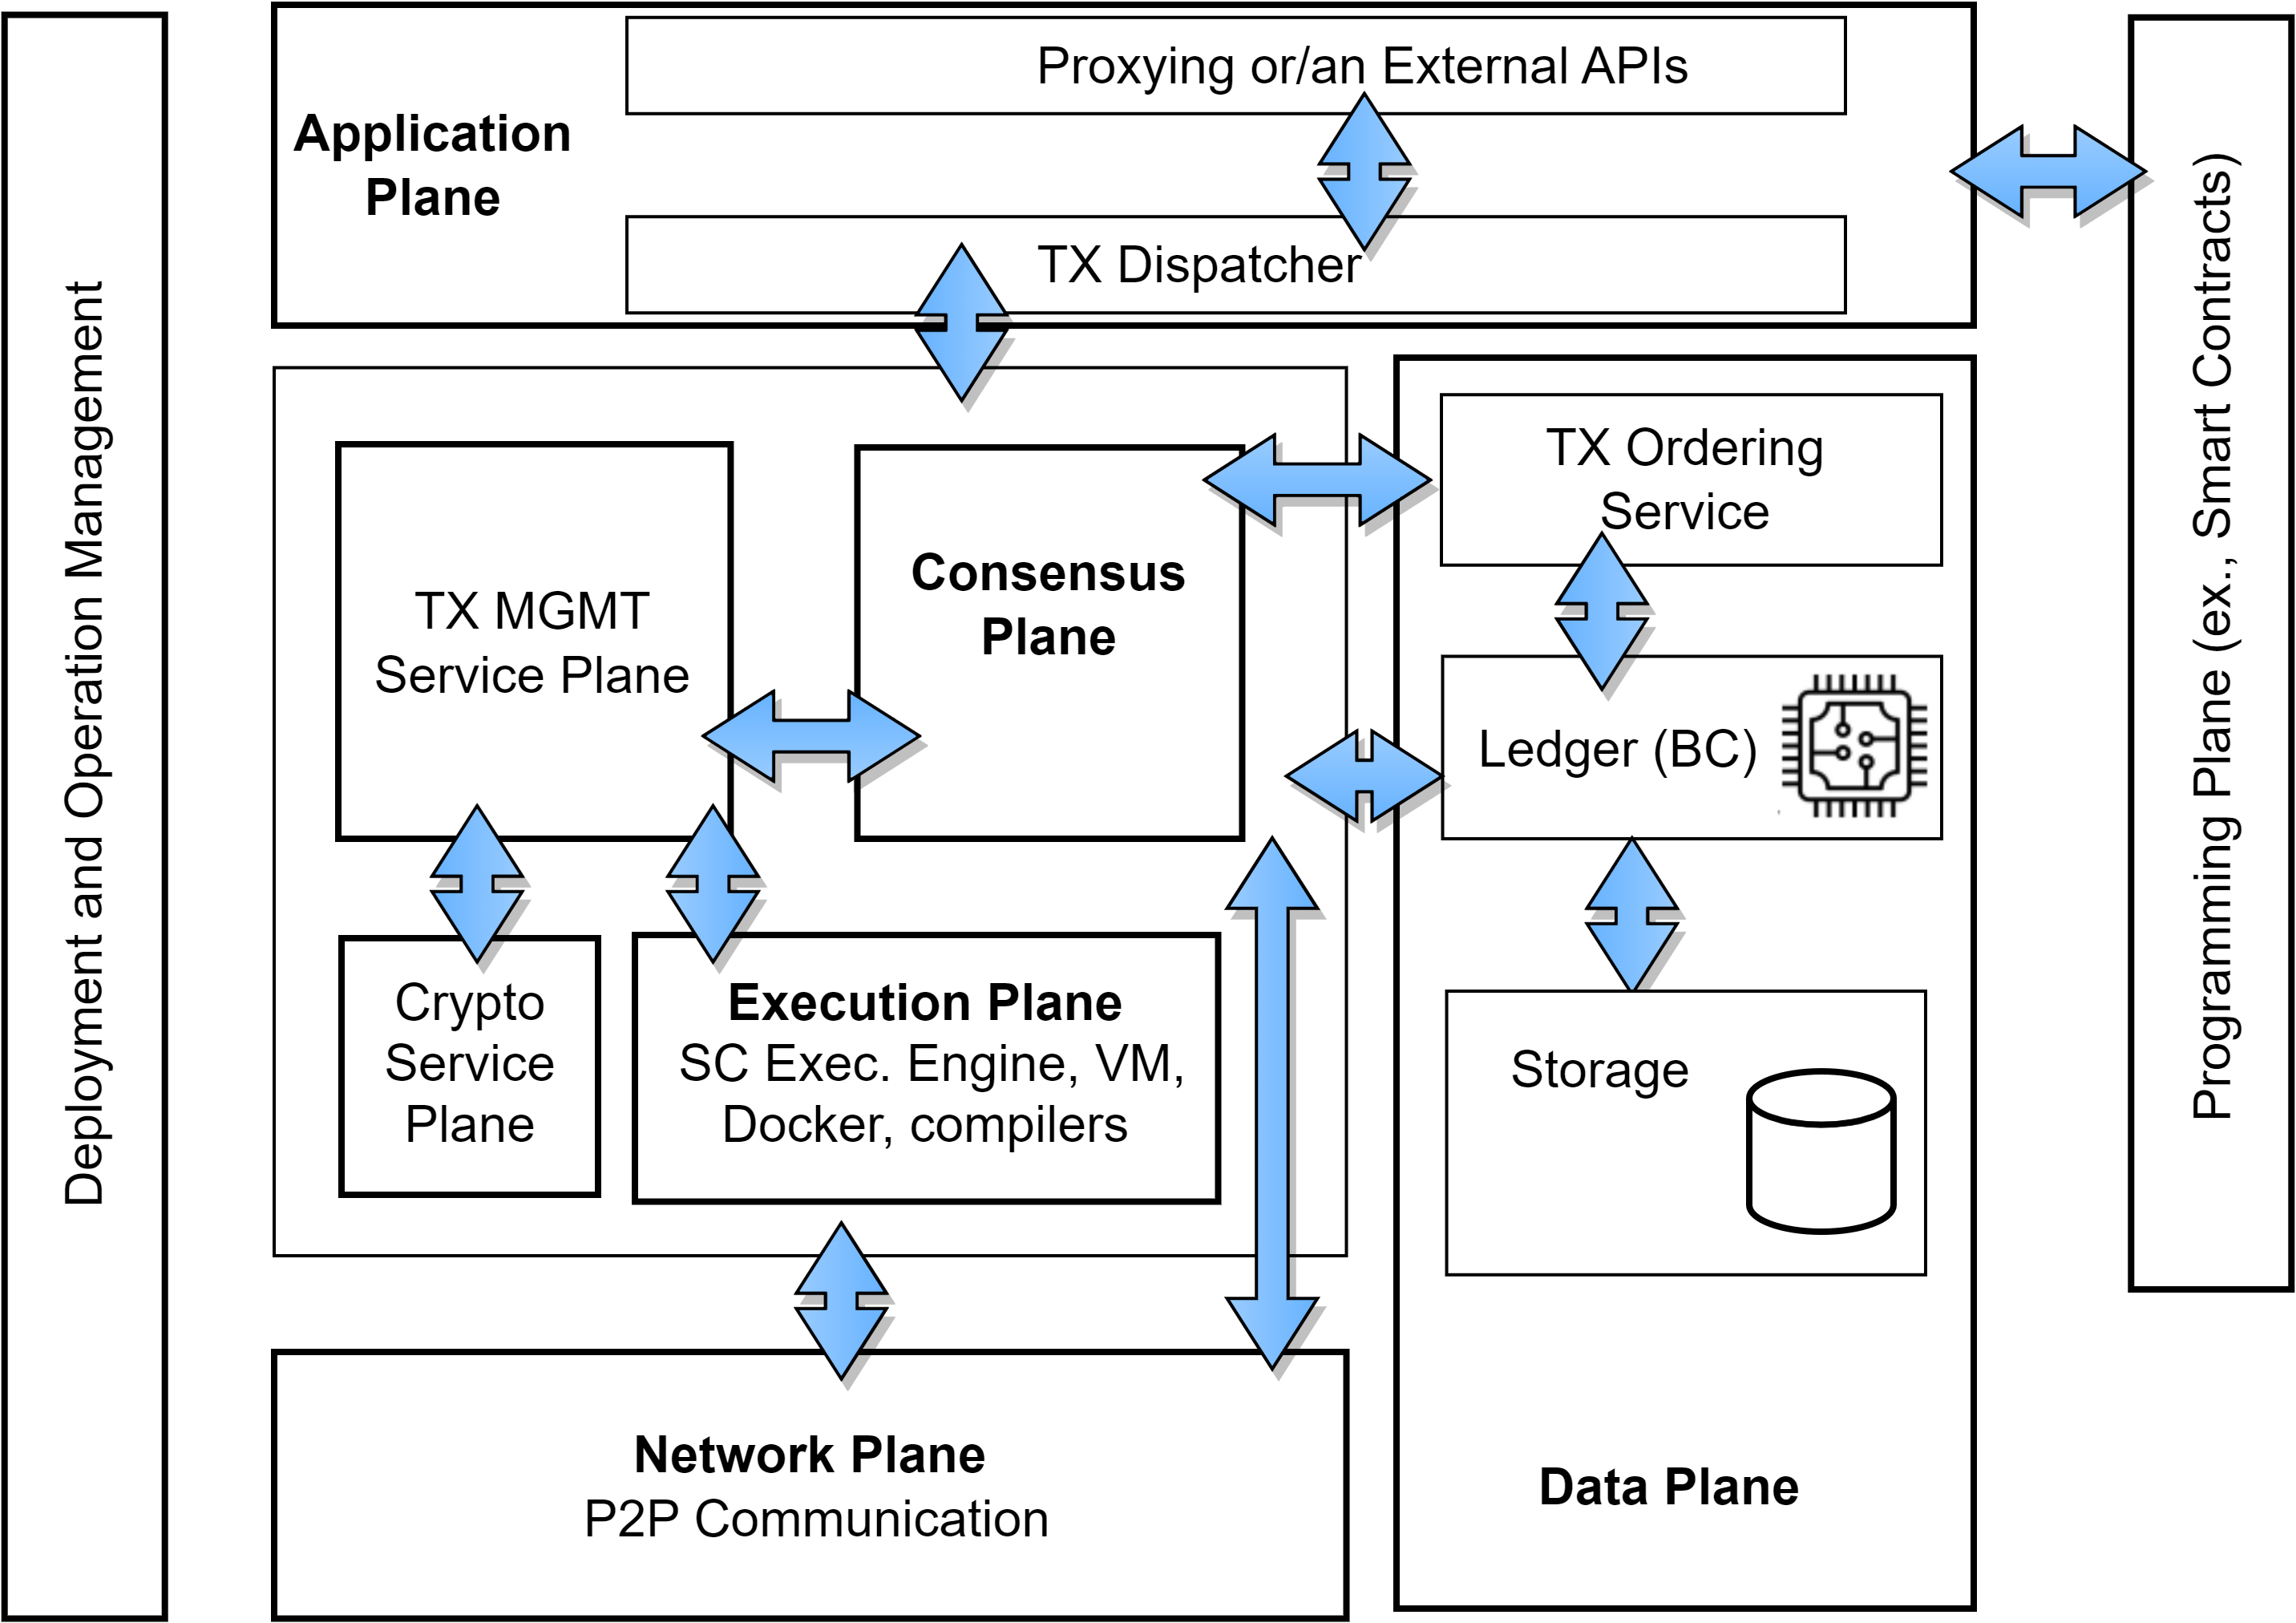
\includegraphics[scale=0.55]{Chapters/Figures/drawio/blockchain_architecture.png}
    \caption{Generic Blockchain Architecture}
    \label{fig:blockchain_architecture}
\end{figure}

When designing a system, it is important to separate concerns and a blockchain is no exception. In figure \ref{fig:blockchain_architecture} is represented a modular specification of an architecture for a generic blockchain with different service planes. % Note that there are various planes related to identification, membership management and access control that only make sense for permissioned blockchains.
This specification derives from the one presented in \cite{systematic_survey_blockchain_systems} which describes the following service planes: application plane, execution plane, data plane, consensus plane and network plane. For each of these planes we present the corresponding explanation while referring to the presented specification.

\paragraph{Application Plane}

The application plane fits on top the blockchain system and supports the integration for applications that are built on top of it, mainly used by the end user. With this, blockchains must have an external API for applications to be able to interact with it. There are many types of applications that could use a blockchain and the most popular are cryptocurrencies.

\paragraph{Execution Plane}

The execution plane is responsible for executing smart contracts on the blockchain. The smart contracts may contain some business logic and be used when validating transactions (see \ref{sec:background:smart_contracts}). This plane is integrated in the \textit{Transaction Management} plane, more specifically in the \textit{Smart Contract Execution Engine}.

\paragraph{Data Plane}

There are many aspects when referring this plane, namely: transaction models, % (such as: \gls{UTXO} or account)
data structures which includes the block structure and Merkle trees, hash functions, encryption algorithms and many others (see \ref{sec:rel_work:dl_ds}). It is responsibility of this plane to define the way that data is stored in the ledger and also the data structures used to represent it. With this, the \textit{Ledger}  and consequently the \textit{Storage} planes are integrated in this plane. Moreover, the hash functions (ex SHA256, etc) and encryption algorithms (RSA, ECC) are extremely important when verifying and validating transactions and also when identifying blocks, thus the \textit{Crypto Services plane} is also integrated. % This layer deals with the issues of different transaction models, namely the \gls{UTXO} and account ones. When we refer to \gls{UTXO}, i.e. transactions owned by a participant that were received but not yet spent, thus the sum of their values reveals the balance of the participant. When a transaction occurs, the peer must reference one of these unspent transactions and the system will validate their ownership and check for double spending. If all these verifications pass then the ownership of the referenced \gls{UTXO} is transferred to the receiver's public key. On the other hand, the account model is more efficient because it updates both accounts (sender and receiver) atomically in one transaction. Moreover, the way that the data of the blockchain is stored in the ledger and the used data structures is also an important aspect when dealing with this layer and so, the \textit{Ledger plane} and consequently the \textit{Storage plane} are integrated in this layer. Lastly, the hash functions (ex SHA256, etc) and encryption algorithms (RSA, ECC) are extremely important when verifying and validating transactions and also when referencing the previous block to form a linked list (blockchain) of ordered blocks, thus the \textit{Crypto Services plane} is also integrated.

\paragraph{Consensus Plane}

The Consensus plane is responsible for ordering transactions/blocks in a way that ensures that every participant contains the same ordered ledger. This is the core plane in a blockchain that solves the common problem to Distributed Systems, namely the consensus problem. There are many consensus algorithms, each of them with different tradeoffs that can be used in different situations based on the type of blockchain and user preferences. In subsection \ref{subsec:arch_service_planes:consensus} is presented the most common consensus algorithms and mechanisms used in blockchains such as: \gls{PoW}, \gls{PoS}, \gls{PoET} and \gls{PBFT}.

\paragraph{Network Plane}

The Network plane is the base plane for all these systems. It implements a \gls{P2P} network used for peer discovery and propagation of transactions and blocks. Depending on the type of blockchain it can have thousands of participants for permissionless or over a hundred for permissioned ones. Either way, the network serves the purpose of transmitting information for the system to be able to reach consensus and so, speed and stability are important characteristics that can affect the performance and efficiency of systems that operate on top of it. It is in this plane that different timing and fault models take place, specifically when referring to the time a message takes to be received or the type of faults the system can handle (see \ref{subsec:arch_service_planes:timing_fault_models}).   % Moreover, it is through this layer that new participants discover and contact others with the intention of joining the system. When analysing different nodes on the network, there are two possibilities: full nodes and light nodes. Full nodes are nodes that participate in the consensus protocol and transaction validation, while in light nodes they mostly act as a client to issue transactions for the system.

\subsection{Timing, Fault Models and Scalability Issues}
\label{subsec:arch_service_planes:timing_fault_models}

% - Timing, Fault and Scalability Issues  (VER P Camponês)   (Pedro)

When we refer to decentralized systems, there are some important characteristics that must be considered. One of them is the time assumption of a system which can be of three types \cite{book_reliable_secure_distributed_programming}: Asynchronous, Synchronous and Partially Synchronous. An \textbf{Asynchronous System} is a system in which there are no assumptions regarding the delay in the delivery of messages. With this, processes do not have access to any sort of physical clock and consequently there are no bounds on processing or communication delays. On the other hand, \textbf{Synchronous Systems} are exactly the opposite of the previous one in the sense that exists an upper bound for computation and communication delays. However, this type of systems do not actually exist. The last model, \textbf{Partially Synchronous} fits in the middle of the two other models in the sense that it is possible to break some timing assumptions for a limited time duration \cite{consensus_partial_synchrony}.

Another important concept is the fault model of a system which can be of three types \cite{book_reliable_secure_distributed_programming}. The \textbf{Byzantine Fault Model} \cite{byzantine_generals_problem} states that a system must be able to defend against malicious attacks. The origin of these attacks might come from the nodes of the system, called as faulty nodes, which is a common case in permissionless blockchains, since there is no control on its participants. The other nodes that follow the protocol are called the correct nodes. Another model is the \textbf{Omission Fault Model} that represents inactive nodes. In this case, this type of nodes choose consciously and not maliciously to not participate in the system. The other nodes, the ones that contribute to the progress of the system are called the active nodes. The third model, the \textbf{Crash Fault Model} stands in the position that every node may realise that some other node has crashed and possibly do something to compensate that loss. The disadvantage of this model is that it is not possible to reliably detect when a node has failed under an asynchronous timing assumption.

Additionally, permissionless blockchains impose another challenge, namely scalability by supporting dynamic membership. With this, it is impossible for the system to expect a certain and fixed number of participants.

\subsection{Consensus Planes and Mechanisms}
\label{subsec:arch_service_planes:consensus}
% - Consensus planes and mechanisms

%  PoW, PoS, PoET, PBFT    (ver que tb aperece no Pedro no Jorge)

As already stated, the Consensus Plane is the core of a blockchain in the sense that consensus is responsible for ensuring that all replicas agree on the same order in which operations are executed, thus achieving \gls{SMR}. In the context of blockchains, the operations corresponds to transactions and all the nodes must validate and execute them in the same order, leading to a consistently replicated ledger. For this purpose, algorithms must comply with the following properties \cite{book_reliable_secure_distributed_programming}: a) termination - every correct process eventually decides a value; b) validity - if a process decides $v$ then $v$ was proposed by some process $p$; c) integrity - no process decides twice; and d) agreement - no two correct processes decide differently. 

Although, when applying consensus in blockchains, the underlying model corresponds to an asynchronous system and so, the FLP Impossibility emerges \cite{flp}. The FLP Impossibility states that there is no deterministic protocol that solves the consensus problem in an asynchronous system where a single process may fail. This means that it is not possible to guarantee all properties of consensus. To circumvent this issue, implementations of consensus algorithms have been relaxed in a way that they can be used to reach consensus (most of the times), but at some cost. Next, we present the most common consensus algorithms applied in blockchains.

\paragraph{\gls{PoW}} Proof-of-Work \cite{pow} is an algorithm that reaches consensus by comparing computer power among the participants. It was initially introduced with the purpose to combat email spam via a computational effort of the sender \cite{pow_email_spam} and is currently used in blockchains, namely in Bitcoin. In fact, Bitcoin uses a \gls{CPU} bound variant in which the core idea of the algorithm is to issue a cryptographic puzzle where the only way to solve it is by generating a nonce, compute a hash and comparing if the hash is inferior with some pre-defined difficulty value. To this process of discovering the correct nonce is called mining. It is used a secured hash function which is pre-image resistant that guarantees that there is no deterministic way of solving the problem. Although this solution is completely fair and decentralized, in the sense that every node can participate, it consumes a lot of energy and has a very low throughput. Also, consistency is not guaranteed because it allows temporary inconsistencies in the ledger (forks on the chain).

\paragraph{\gls{PoS}} To mitigate the disadvantages of \gls{PoW}, Proof-of-Stake \cite{pow_vs_pos_eval_performance_and_security} is introduced as a relatively fast and energy-saving consensus algorithm. In this algorithm, nodes that create and validate blocks need to have stake by depositing coins in an escrow account. After this, a group of nodes is selected to participate in the consensus (based on the amount of stake). But, in case of incorrect or malicious actions, a node (or stakeholder) can loose part or all of its stake. It is the purpose of this algorithm to incentivate good behaviour from nodes and thus, mitigating attacks on the network. However, there exists some tradeoffs like the lack of decentralization of the base of trust based on the elected participants. Also, \gls{PoS} comes in different flavours, such as: \gls{DPoS}, \gls{LPoS}, \gls{ZPoS} and \gls{PPoS}. 

\paragraph{\gls{PoET}} Proof-of-Elapsed-Time \cite{poet_security_analysis} is another approach in reaching consensus with the same benefits of \gls{PoS}. In this case, it is very similar to \gls{PoW} in the sense that it relies on the concept of electing a leader in each round to propose the next block to the distributed ledger. This algorithm was invented by Intel by leveraging the \gls{TEE}, namely the \gls{SGX} capability. With this algorithm, a validator executes a lottery function and waits for the specified time returned by that function. This algorithm is secured because the execution is done within the processor secure enclave and it is fair and easy for any participant to verify it. The disadvantage of this approach is that a node needs a \gls{CPU} with \gls{SGX} capability to participate in the algorithm.

\paragraph{\gls{PBFT}} The \gls{PBFT} \cite{pbft} algorithm was introduced by Miguel Castro and Barbara Liskov in 1999 and is a consensus protocol that can tolerate up to $f$ Byzantine Faults in a system with $3f + 1$ replicas. This algorithm evolves by rounds and it starts by a client request to the primary replica. Then, the primary starts the PRE-PREPARE phase by multicasting a message to every other replica and the PREPARE and COMMIT phases follow it. Finally, the protocol terminates when the client receives $f + 1$ replies from different replicas. Although this is fast at achieving consensus and solves all the above tradeoffs, it is limited by scalability because it requires a fixed membership and any alterations to it must be decided as any other value, thus being very inefficient for permissionless blockchains.


\section{Summary}
\label{sec:background:summary}

In this chapter, we presented the background topics that cover this thesis, including the definition of a \gls{DL}, different models of blockchains and an overview of the architecture of those systems while focusing on the consensus plane and the different consensus mechanisms and tradeoffs. Additionally, we analysed how different blockchains implemented smart contracts and also giving an intuition on how they could be used to permit the modification of the consensus mechanism at runtime. % Also, we presented a comparative analysis of the implemented consensus plane for different blockchain platforms. % Moreover, we explored the \gls{CUP} model and how it could be used for building a consensus mechanism for the permissionless model that fits the objectives of this thesis.



%
% Please note that
% \begin{center}
%   \textbf{\large this package and template are not official for FCT/NOVA}.
% \end{center}



% \printbibliography[heading=subbibliography, segment=\therefsegment, title={\bibname\ for chapter~\thechapter}]
